\section{Protocol design}

TCP/IP consists of two primary protocols: the Transmission Control Protocol, which manages data flow between two endpoints, and the Internet Protocol, which handles the addressing and routing of packets.

TCP is a connection-based protocol that requires a stable connection before data transfer can occur. This connection is established through a three-way handshake process. Initially, a computer sends a SYN (synchronize) bit to the server to initiate a connection. The server acknowledges this by replying with a packet that contains both an SYN bit and an ACK (acknowledgment) bit. To complete the handshake, the initiating computer sends an ACK bit back to the server confirming that the connection has been setup successfully. With this process completed, data can be transmitted reliably. If data is lost or corrupted during transmission, it is re-sent, creating a connection that is effectively lossless (See Figure \ref{fig:tcp}).
\begin{figure}
    \centering
    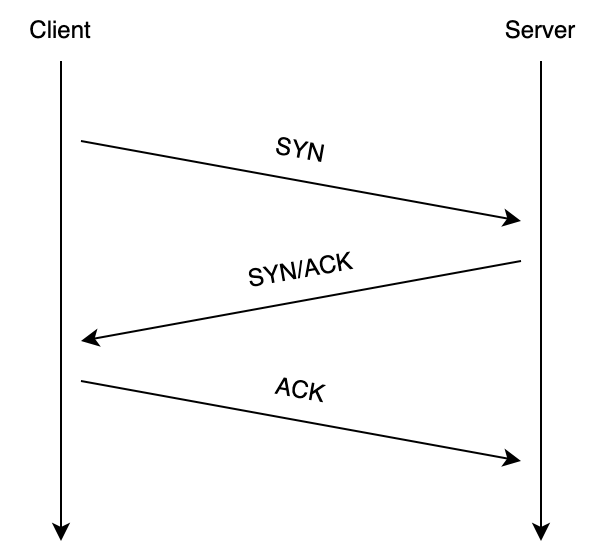
\includegraphics[width=1\linewidth]{attachments/tcp_ip_protocol.drawio.png}
    \caption{TCP Three-Way Handshake}
    \label{fig:tcp}
\end{figure}